\chapter{Legal Origins and Finance}
\label{ch:llsv}

\section{Law and finance}

In 1997 and 1998 Rafael La Porta, Florencio L\'opez-de-Silanes, Andrei Shleifer and Robert Vishny published two papers that changed how economists think about law \citep{llsv1997,llsv1998}. Robert Vishny, a colleague at Chicago Booth, and his coauthors asked a simple question: do the legal rules that protect outside investors differ across countries, and if so, do the differences explain why some countries have large capital markets and dispersed ownership while others have small markets and concentrated ownership? Their answer was yes, and the differences were organised by legal origin. Countries whose commercial law descends from English common law protected shareholders and creditors more strongly than those whose law descends from French civil law, with German and Scandinavian civil law countries in between. Strong protection was associated with larger equity markets, more initial public offerings and more dispersed ownership.\index{La Porta, L\'opez-de-Silanes, Shleifer and Vishny}\index{legal origins}

The papers launched a literature of thousands of articles, influenced the World Bank's \emph{Doing Business} reports, and provoked fierce criticism. This chapter explains what the authors found, how they measured it, what the critics said, and how a Bayesian approach to the evidence clarifies what we can and cannot conclude.

\section{Measuring investor protection}

\subsection{The antidirector rights index}

\emph{Law and Finance} coded the company and bankruptcy laws of forty-nine countries. For shareholders, the authors constructed an antidirector rights index by adding one point for each of six provisions that strengthen minority shareholders against managers and controlling shareholders: shareholders can vote by mail; shares are not blocked before a shareholders' meeting; cumulative voting or proportional representation of minorities on the board is allowed; there is a legal mechanism for oppressed minorities to challenge directors' decisions; shareholders have pre-emptive rights to new issues; and the share of capital needed to call an extraordinary meeting is ten per cent or less. The index ranges from zero to six. Common law countries averaged about four, French civil law countries about two and a third.\index{antidirector rights index}

\subsection{Creditor rights}

For creditors, the index added one point for each of four provisions: restrictions on entering reorganisation, such as creditor consent; no automatic stay on secured assets; secured creditors paid first in liquidation; and management does not stay in control during reorganisation. Common law countries again scored higher on average, though the pattern was less clean; German origin countries also protected creditors strongly.

\subsection{Enforcement}

Laws on the books matter only if enforced. The authors used survey-based measures of the efficiency of the judicial system, the rule of law, corruption, the risk of expropriation and the quality of accounting standards. Here the ranking was different: Scandinavian and German origin countries scored highest, French origin countries lowest, with common law countries in between but closer to the top.

\section{The findings}

The central empirical results can be summarised in three statements.
\begin{enumerate}[label=(\roman*)]
\item Legal origin predicts investor protection: common law countries have stronger protections than French civil law countries, controlling for income per capita.
\item Investor protection predicts financial development: countries with stronger protection have larger stock markets relative to GDP, more listed firms per capita and more initial public offerings.
\item Weak protection is associated with concentrated ownership: where minority shareholders are poorly protected, large shareholders hold larger stakes, plausibly as a substitute for legal protection.
\end{enumerate}
In a 2008 survey in the \emph{Journal of Economic Literature}, La Porta, L\'opez-de-Silanes and Shleifer extended the argument, proposing that legal origin represents a style of social control of economic life \citep{lls2008}. The common law supports private market outcomes and resolves disputes; the civil law implements state policy and regulates. They reported that legal origin predicts not only financial rules but labour regulation, the formalism of judicial procedure, government ownership of banks, entry regulation and government ownership of the media.

\subsection{Courts}

Djankov, La Porta, L\'opez-de-Silanes and Shleifer's paper \emph{Courts} in 2003 studied the procedures for two simple disputes, evicting a tenant for non-payment of rent and collecting a bounced cheque, in one hundred and nine countries \citep{djankov2003}. They constructed an index of procedural formalism from the requirements for written submissions, professional lawyers, legal justification of decisions, statutory regulation of evidence and appeals. Formalism was systematically higher in civil law countries, and higher formalism was associated with longer expected duration of proceedings, less consistency, less honesty and less fairness in judicial decisions as assessed by survey respondents. The paper connects directly to Chapter~\ref{ch:commoncivil}: the civil law's preference for written evidence and its fixed rules of proof are measured components of formalism.\index{formalism}

\subsection{Why origins differ}

Glaeser and Shleifer offered a historical explanation for the divergence \citep{glaeser2002}. Their mechanism is the level of peace and order. In medieval England, a relatively peaceful country with weaker local magnates, it was possible to entrust disputes to local juries, independent of the king. In France, a more violent environment with powerful local magnates led to a centralised system of royal judges applying written law, which protected litigants from local coercion. Each system was efficient for its environment, and each was transplanted to colonies where the original rationale no longer applied.

\section{The critics}

\subsection{Measurement}

Holger Spamann recoded the antidirector rights index from primary legal sources and found many coding errors in the original \citep{spamann2010}. With the corrected index, the difference between common law and civil law countries was substantially smaller and the relation between the index and financial development weaker. The authors had revised the index in later work. The episode illustrates a general problem: legal rules are complex, and translating them into binary indicators requires judgments about what counts, judgments that can be made differently by competent lawyers.

\subsection{Identification}

Legal origin was not randomly assigned. Countries acquired their legal systems through colonisation, conquest or imitation, and the same historical processes brought language, religion, institutions, settlers and trading relationships. Acemoglu, Johnson and Robinson argued that the institutions colonisers established depended on the disease environment and on whether they settled or extracted \citep{acemoglu2001}. Klerman, Mahoney, Spamann and Weinstein showed that once colonial history is controlled for, legal origin explains much less: British colonies differ from French ones in many ways besides law \citep{klerman2011}. Rajan and Zingales documented that financial development was not monotonic over the twentieth century; in 1913 France had a larger stock market relative to GDP than the United States, and the reversal came later \citep{rajan2003}. If legal origin were the dominant cause, such reversals would be hard to explain.

\subsection{Politics}

Mark Roe argued that the political economy of the twentieth century, in particular the strength of social democracy and labour after the World Wars, explains ownership concentration better than legal origin \citep{roe2003}. Where politics favoured employees, managers aligned with labour against shareholders, and concentrated owners were needed to discipline managers.

\section{A Bayesian assessment}

How should one weigh this evidence? The question is a classic case of inference with a small sample, measurement error and confounding.

\subsection{The sample}

There are about fifty countries in the original studies and perhaps one hundred and fifty in later ones. Legal origin takes a few values. Within each origin, countries vary enormously in income, history and institutions. Many plausible confounders are correlated with origin. With so few observations and so many potential confounders, any single regression is fragile, and the reported standard errors understate uncertainty about the model.

\subsection{Model uncertainty}

Bayesian model averaging addresses model uncertainty directly. Rather than choosing one set of controls, the analyst places a prior over models, each defined by a set of included variables, computes the posterior probability of each model given the data, and averages the estimated effect of legal origin across models weighted by their posterior probabilities. Sala-i-Martin, Doppelhofer and Miller applied a version of this approach to cross-country growth regressions and found that only 18 of 67 proposed determinants of growth were robust \citep{sala2004}. A similar exercise for financial development would report a posterior distribution for the effect of legal origin that accounts for uncertainty about which confounders matter. If the posterior probability that origin matters, given colonial history, settler mortality and the other candidates, is high, the legal origins thesis survives. If the effect's posterior mass straddles zero across plausible models, the evidence is weaker than the original papers suggested.\index{Bayesian model averaging}

\subsection{Measurement error}

Spamann's recoding suggests that the indices contain substantial error. In a Bayesian measurement model, the observed index is a noisy indicator of a latent level of protection, with error variance estimated from the disagreement between codings. The effect of latent protection on financial development is then estimated with appropriate attenuation corrections. Classical measurement error in a single regressor biases its coefficient toward zero, so correcting for it could strengthen the estimated effect of protection on development, even as recoding weakens the association between protection and origin.

\subsection{Hierarchical shrinkage}

Within each legal origin family, country estimates of protection or of its effects vary. A hierarchical model pools information within families while allowing each country its own value. Figure~\ref{fig:shrinkage} illustrates the effect on simulated data: raw country estimates, which are noisy, are pulled toward their family means, more strongly for countries with less precise estimates. The family means themselves are usually estimated more precisely than any single country. This approach, standard in Bayesian analysis of grouped data, is well suited to comparative law, where the groups are legal families and the units are countries. It also allows the data to tell us how different the families really are: if the between-family variance is small relative to within-family variance, legal origin explains little.

\begin{figure}[t]
\centering
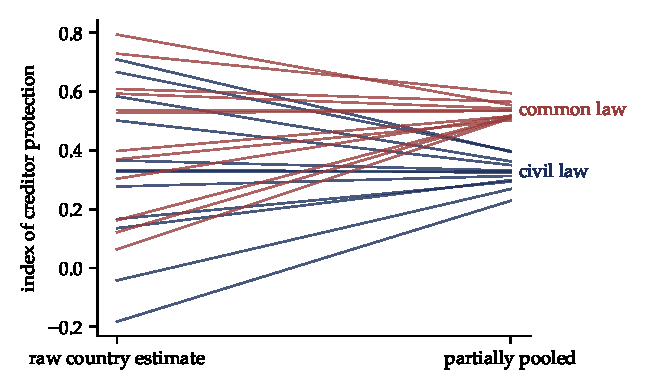
\includegraphics[width=\linewidth]{fig_shrinkage}
\caption{Partial pooling of country level estimates of creditor protection within two legal families, using simulated data. Raw estimates on the left are shrunk toward their family means, giving the partially pooled estimates on the right.}
\label{fig:shrinkage}
\end{figure}

\section{What we can conclude}

Taking the evidence as a whole, a reasonable posterior is roughly as follows. Legal rules protecting outside investors matter for financial development; this is supported by within country evidence from legal reforms as well as cross-country comparisons. Legal origin is correlated with those rules, but much less sharply than the original codings suggested, and it is confounded with other features of colonial history. The broader claim that legal origin represents a style of social control with wide consequences is plausible but less firmly established. And the mechanisms by which law affects finance, through courts, regulators, private enforcement and political economy, are only partly understood.

Two points from the debate are especially relevant to this book. First, enforcement matters as much as rules, and enforcement depends on courts. A rule protecting minority shareholders is worth little if courts take years to decide cases or decide them inconsistently. The procedural formalism documented in \emph{Courts} is a direct measure of how hard it is to obtain a decision. Second, the information that courts generate, in the form of reasoned decisions, is a public good that shapes behaviour. A system whose decisions are predictable reduces litigation and makes contracting cheaper. The Bayesian view of precedent in Chapter~\ref{ch:commoncivil} explains why: precedent is accumulated data about the law, and its value depends on its volume and consistency.

\section{From legal origin to legal technology}

The legal origins literature studied systems as they were in the late twentieth century. Technology is now changing how both traditions operate. Electronic filing, online dispute resolution and machine analysis of judgments reduce the cost of information about law and about cases. If formalism is costly because it slows proceedings and raises the cost of legal services, technology may reduce the penalty for formalism; if precedent is valuable because it accumulates information, machine learning may extract that information more effectively. The comparative advantage of each tradition may shift. Statute based rules are easier to formalise, as Catala shows; precedent based systems produce more data for learning. Chapter~\ref{ch:india} examines how a common law system under extreme load is responding with technology, and Chapter~\ref{ch:lean} how formal verification fits each tradition.

\section*{Notes and Questions}
\addcontentsline{toc}{section}{Notes and Questions}
\begin{enumerate}[label=\arabic*.]
\item List the six components of the antidirector rights index. For one country you know well, code each component and compare your coding with that in the original paper.
\item Suppose the observed index $I_c$ equals latent protection $P_c$ plus error with variance $\sigma^2$, and two independent codings differ by one point in mean squared difference. Estimate $\sigma^2$. By how much would the coefficient of $I_c$ in a regression of market size on $I_c$ be attenuated if the variance of $P_c$ were two?
\item Design a Bayesian model averaging exercise for the effect of legal origin on stock market capitalisation. Which candidate controls would you include? What prior over models?
\item Rajan and Zingales's great reversal shows that France's stock market was relatively large in 1913. Is this evidence against the legal origins thesis? What would a defender say?
\item The \emph{Courts} paper measured formalism for eviction and cheque collection. Propose a similar measure for the speed and consistency of decisions on commercial contracts, and explain how you would estimate it.
\item Explain why a hierarchical model with legal families as groups can reveal whether legal origin matters. What would you conclude if the posterior for between-family variance were concentrated near zero?
\end{enumerate}

\section*{Further reading}
The original papers \citep{llsv1997,llsv1998}; the 2008 survey \citep{lls2008}; \emph{Courts} \citep{djankov2003}; Spamann's recoding \citep{spamann2010}; Klerman and colleagues on colonial history \citep{klerman2011}; Roe on politics \citep{roe2003}.
